% ─────────────────────────────────────────────────────────────────
\section{Dataset Separability Analysis}
\label{sec:analysis}
% ─────────────────────────────────────────────────────────────────

Before training any classifier we conduct a thorough statistical separability
study at two resolutions --- the 1\,000-node SSL graphs that are the primary
training data (Section~\ref{sec:analysis:graph}), and the full-resolution VTK
meshes as a validation of the subsampling step
(Section~\ref{sec:analysis:vtk}).
Section~\ref{sec:analysis:compare} then quantifies how much information is
lost in the FPS pipeline.

% ─────────────────────────────────────────────────────────────────
\subsection{Graph-level Separability (1k-node SSL Graphs)}
\label{sec:analysis:graph}
% ─────────────────────────────────────────────────────────────────

\subsubsection{Sliced Wasserstein: Shape vs.\ Features vs.\ Joint}
\label{sec:analysis:graph:sw}

We compute the Sliced Wasserstein (SW) distance on three views of each
1\,000-node graph:
\begin{itemize}
  \item \textbf{SW(xyz)}: 3D coordinates only --- measures how different the
        point-cloud \textit{shapes} are between classes.
  \item \textbf{SW(feat)}: electrostatic features + normals
        (\textit{Potential\_norm, NormalPot\_norm, $n_x, n_y, n_z$}) ---
        measures distributional difference in the surface chemistry.
  \item \textbf{SW(joint)}: all 8 features combined --- the full 8D
        per-vertex distribution.
\end{itemize}

\begin{figure}[ht]
  \centering
  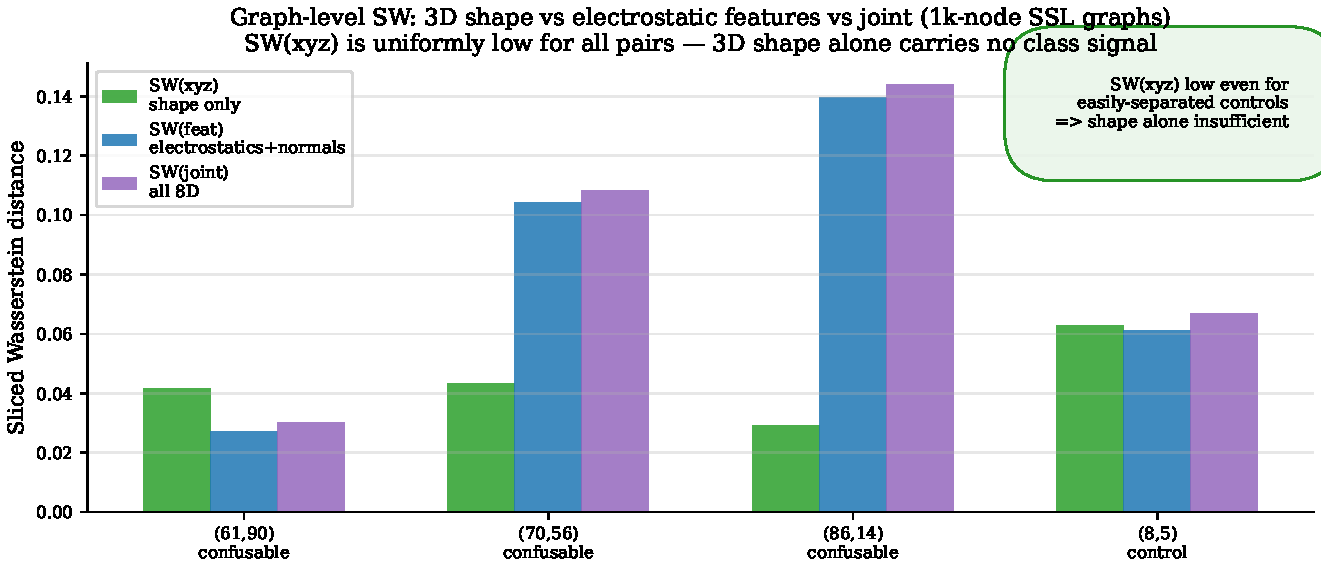
\includegraphics[width=\linewidth]{figures/separability_graph_sw.pdf}
  \caption{Graph-level Sliced Wasserstein for the three confusable pairs
           and a control pair.
           SW(xyz) is uniformly low ($<$0.065) for all pairs including
           controls, confirming that 3D surface shape alone carries no
           class-discriminating signal.
           SW(feat) correctly distinguishes easy pairs (0.10--0.14) from
           the near-inseparable pair (61,\,90) (0.027).}
  \label{fig:graph_sw}
\end{figure}

\begin{table}[ht]
  \centering
  \caption{Graph-level SW distances on 1\,000-node SSL graphs.}
  \label{tab:graph_sw}
  \begin{tabular}{lcrrrr}
    \toprule
    \textbf{Pair} & \textbf{Type} & \textbf{SW(xyz)} & \textbf{SW(feat)} & \textbf{SW(joint)} \\
    \midrule
    (61,\,90) & confusable & 0.042 & 0.027 & 0.030 \\
    (70,\,56) & confusable & 0.043 & 0.104 & 0.108 \\
    (86,\,14) & confusable & 0.029 & 0.140 & 0.144 \\
    (8,\,5)   & control    & 0.063 & 0.061 & 0.067 \\
    \bottomrule
  \end{tabular}
\end{table}

\textbf{Key finding:} SW(xyz) ranges from 0.029 to 0.063 across \textit{all}
pairs, including the easily separable controls.
The electrostatic features, not the surface geometry, carry the discriminating
signal.
For pair (61,\,90), even SW(feat) is only 0.027 --- lower than the control
pair (8,\,5) at 0.061 --- confirming near-inseparability at the feature level.

\subsubsection{Spatial Autocorrelation: Moran's I}
\label{sec:analysis:graph:moran}

Moran's I quantifies the spatial autocorrelation of a feature on the surface
graph: high $I$ means nearby vertices have similar values (smooth pattern),
low $I$ means values are spatially random.
We compute $I$ per protein and report the mean over all 12 studied classes,
plus the per-pair difference $|\Delta I|$ which indicates different spatial
patterning between classes.

\begin{figure}[ht]
  \centering
  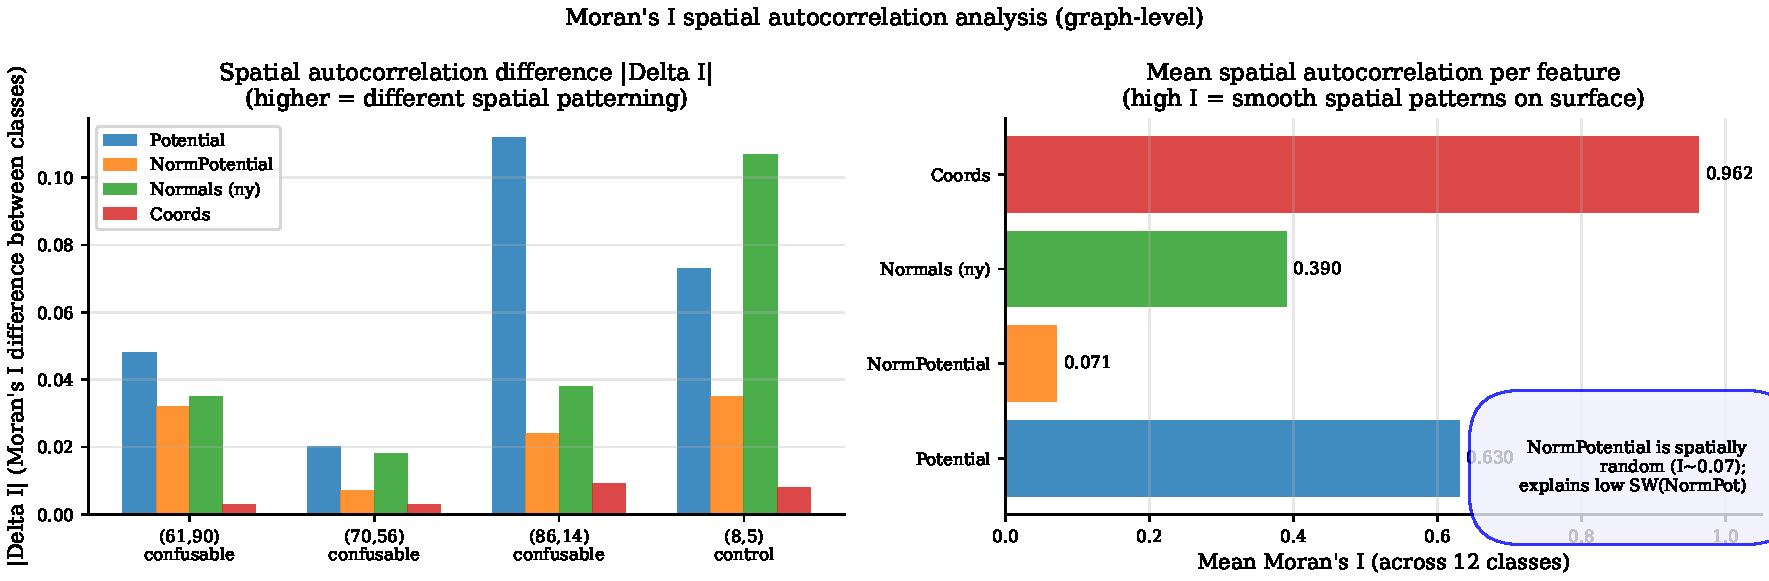
\includegraphics[width=\linewidth]{figures/separability_moran.pdf}
  \caption{Left: $|\Delta I|$ per feature for each pair.
           Potential shows the largest spatial patterning difference,
           especially for (86,\,14) ($|\Delta I| = 0.112$).
           Right: mean Moran's I per feature across all 12 classes.
           NormalPotential is nearly spatially random ($I \approx 0.07$);
           coordinates are very smooth ($I \approx 0.96$).}
  \label{fig:moran}
\end{figure}

The spatial autocorrelation analysis reveals:
\begin{itemize}
  \item \textit{Potential} ($I \approx 0.63$, $|\Delta I|$ up to 0.112):
        large charged patches cluster on the surface; different families
        have different patch arrangements.
  \item \textit{NormalPotential} ($I \approx 0.07$): nearly spatially
        random, consistent with its low KS and SW values.
  \item \textit{Normals} ($I \approx 0.39$): moderately autocorrelated,
        reflecting curvature patches.
  \item \textit{Coordinates} ($I \approx 0.96$): very smooth by
        construction; $|\Delta I| \leq 0.009$ for all pairs, confirming
        that normalised surface coordinates carry no inter-class signal.
\end{itemize}

\subsubsection{Patch-SVM vs.\ Global-SVM on Graphs}
\label{sec:analysis:graph:svm}

To test whether the \textit{spatial arrangement} of features (rather than
their marginal statistics) is what the GNN needs, we compare two protein-level
SVMs:
\begin{itemize}
  \item \textbf{Global-SVM (32D)}: mean, std, skewness, kurtosis,
        25th/75th-percentile of each of the five per-vertex features --- purely
        distributional, no spatial information.
  \item \textbf{Patch-SVM (512D)}: mean feature vector of each of the 64
        geodesic-Voronoi patches, concatenated --- encodes spatial layout.
\end{itemize}

\begin{figure}[ht]
  \centering
  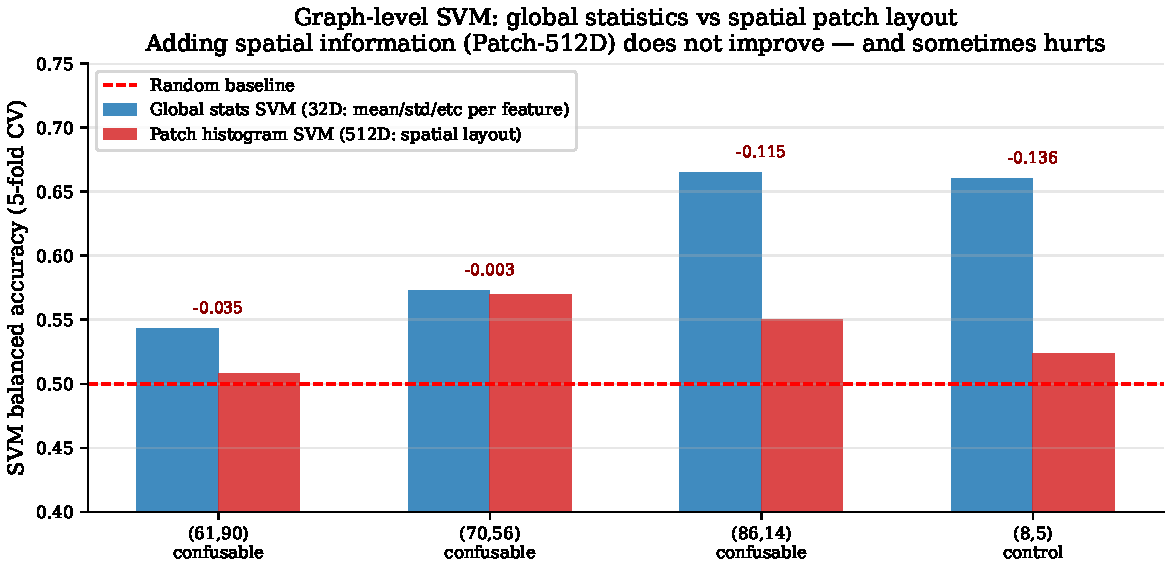
\includegraphics[width=\linewidth]{figures/separability_graph_svm.pdf}
  \caption{Global-SVM (32D) vs.\ Patch-SVM (512D) balanced accuracy on
           1\,000-node graphs.
           The delta annotation shows how much the patch layout adds.
           For all pairs, adding spatial information either gives no gain
           or actively hurts, ruling out spatial arrangement as the
           missing discriminating signal.}
  \label{fig:graph_svm}
\end{figure}

The patch-based SVM is consistently \textit{worse} than the global-statistics
SVM for all pairs.
This counter-intuitive result suggests the 64-patch histogram is too
high-dimensional for the small per-class sample count (SVM overfits to
irrelevant spatial variation), and that the discriminating information is
entirely captured by the marginal feature distributions.

% ─────────────────────────────────────────────────────────────────
\subsection{Full-resolution Analysis (VTK Meshes)}
\label{sec:analysis:vtk}
% ─────────────────────────────────────────────────────────────────

We repeat the separability analysis on the full-resolution VTK meshes
($\approx$10\,676 vertices per protein) to validate the 1k-subsampling step
and to extend the KS and SW analyses to the normalised coordinate axes.

\subsubsection{Vertex-level KS Test (All 8 Features)}
\label{sec:analysis:vtk:ks}

We pool all vertex values across proteins in each class and compute the
two-sample Kolmogorov--Smirnov (KS) statistic.
The normalised coordinates ($x_\text{norm}, y_\text{norm}, z_\text{norm}$)
are obtained by centring each protein at the origin and scaling to unit
maximum absolute value before pooling.

\begin{figure}[ht]
  \centering
  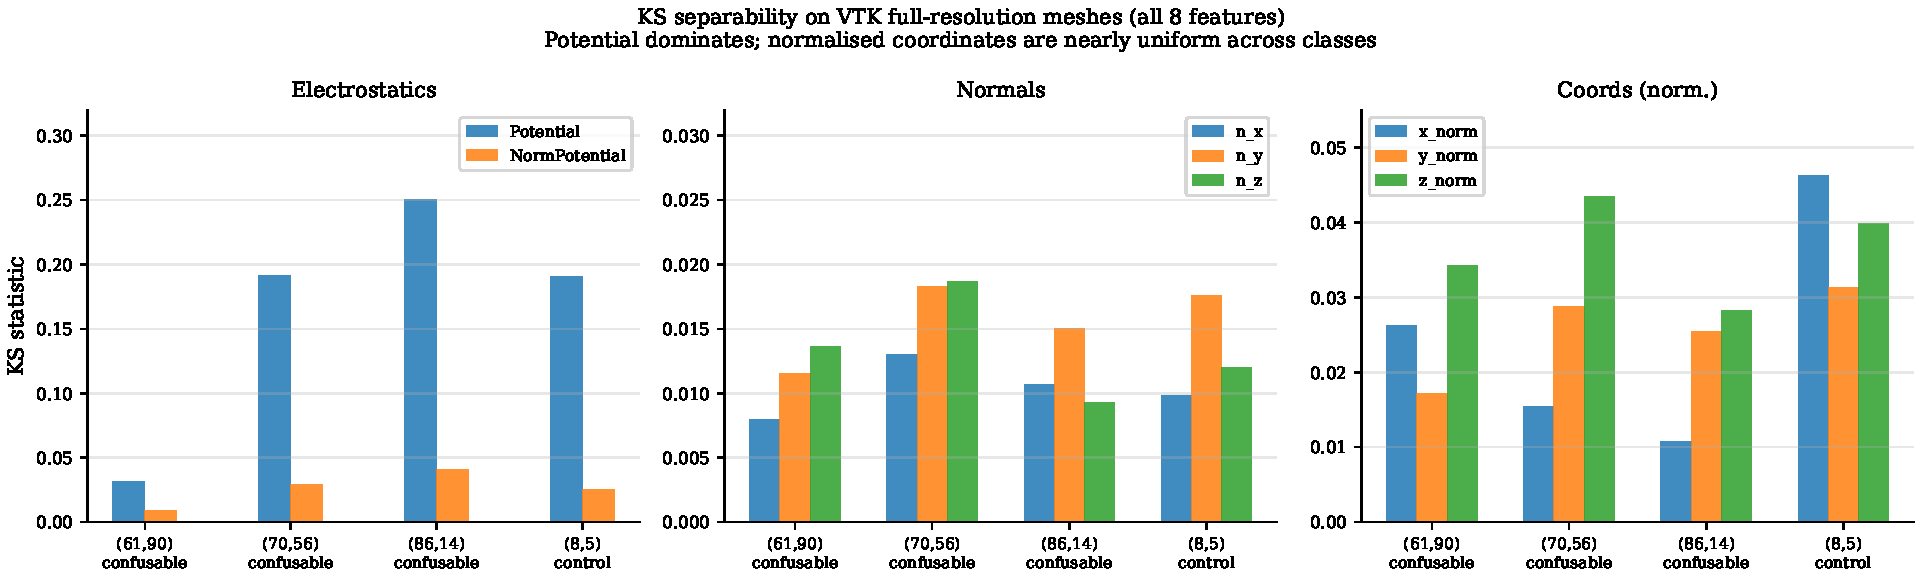
\includegraphics[width=\linewidth]{figures/separability_ks.pdf}
  \caption{KS statistic for all 8 features grouped into three panels:
           electrostatics (left), normals (centre), normalised coordinates
           (right).
           Coordinate KS values (0.01--0.04) are near-zero and comparable
           across confusable and control pairs --- shape marginals do not
           separate classes.}
  \label{fig:ks}
\end{figure}

\begin{table}[ht]
  \centering
  \caption{KS statistics (VTK vertex-level, full resolution).
           Coordinate columns are for per-protein normalised coordinates.}
  \label{tab:ks}
  \begin{tabular}{lcccccccc}
    \toprule
    \textbf{Pair} & \textbf{Pot} & \textbf{NormPot} & $n_x$ & $n_y$ & $n_z$
                  & $x_n$ & $y_n$ & $z_n$ \\
    \midrule
    (61,\,90) & 0.031 & 0.009 & 0.008 & 0.012 & 0.014 & 0.026 & 0.017 & 0.034 \\
    (70,\,56) & 0.192 & 0.029 & 0.013 & 0.018 & 0.019 & 0.015 & 0.029 & 0.043 \\
    (86,\,14) & 0.250 & 0.041 & 0.011 & 0.015 & 0.009 & 0.011 & 0.026 & 0.028 \\
    (8,\,5) ctrl & 0.190 & 0.025 & 0.010 & 0.018 & 0.012 & 0.046 & 0.031 & 0.040 \\
    \bottomrule
  \end{tabular}
\end{table}

The coordinate KS values (0.011--0.046) are uniformly small and show no
consistent pattern between confusable and control pairs: the control (8,\,5)
has \textit{higher} coordinate KS than the confusable (86,\,14), confirming
that coordinate marginals carry no reliable class signal.

\subsubsection{Sliced Wasserstein (VTK, All 5 Components)}
\label{sec:analysis:vtk:sw}

\begin{figure}[ht]
  \centering
  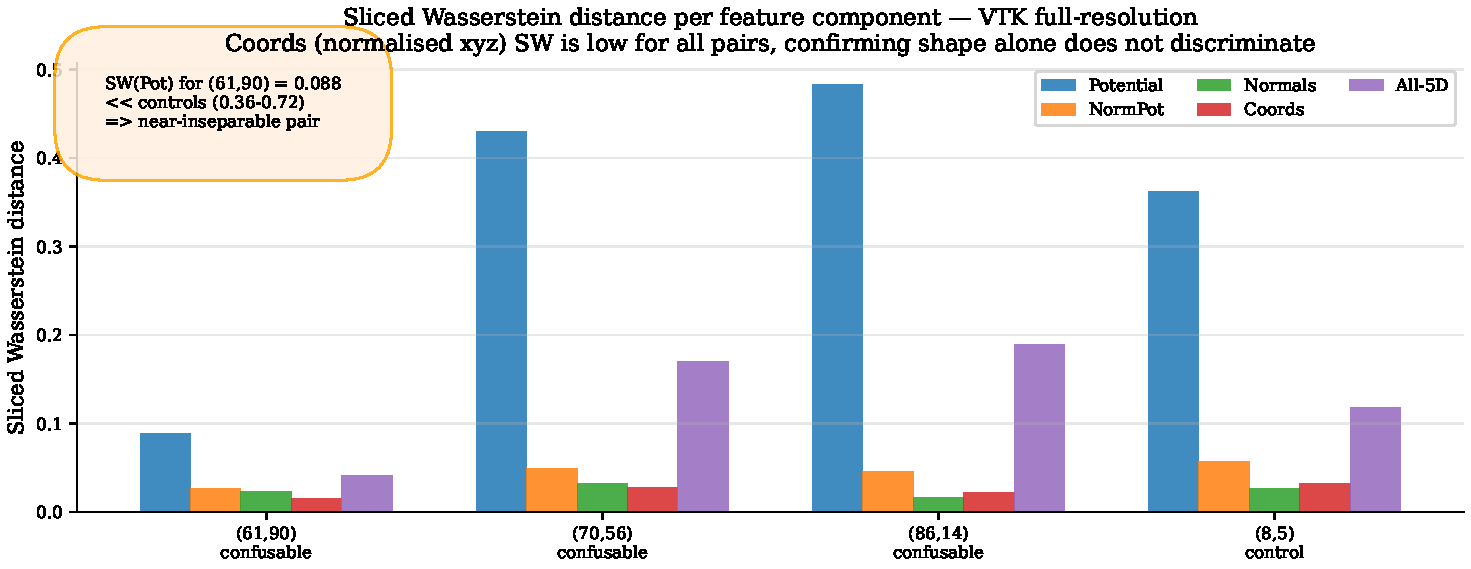
\includegraphics[width=\linewidth]{figures/separability_sw.pdf}
  \caption{VTK Sliced Wasserstein per component.
           The newly added \textit{Coords} column confirms SW(Coords)
           $\leq$0.033 for all pairs --- well below SW(Potential) for
           any separable pair.}
  \label{fig:sw}
\end{figure}

\begin{table}[ht]
  \centering
  \caption{Sliced Wasserstein distances (full-resolution VTK, 5 components).}
  \label{tab:sw}
  \begin{tabular}{lcrrrrrr}
    \toprule
    \textbf{Pair} & \textbf{Type} & \textbf{SW(Pot)} & \textbf{SW(NormPot)}
                  & \textbf{SW(Nrm)} & \textbf{SW(Coords)} & \textbf{SW(All-5D)} \\
    \midrule
    (61,\,90) & confusable & 0.088 & 0.027 & 0.023 & 0.015 & 0.042 \\
    (70,\,56) & confusable & 0.430 & 0.050 & 0.032 & 0.028 & 0.170 \\
    (86,\,14) & confusable & 0.483 & 0.046 & 0.017 & 0.022 & 0.189 \\
    (8,\,5)   & control    & 0.362 & 0.057 & 0.027 & 0.032 & 0.118 \\
    \bottomrule
  \end{tabular}
\end{table}

\subsubsection{Protein-level SVM (Full-res VTK)}
\label{sec:analysis:vtk:svm}

We compute 30D global-statistics vectors per protein (mean, std, skewness,
kurtosis, 25th/75th-percentile of each of the five per-vertex features) and
train a linear SVM with 5-fold cross-validation on the full-resolution meshes.
Results appear in Figure~\ref{fig:resolution} alongside the 1k-graph results.

% ─────────────────────────────────────────────────────────────────
\subsection{Comparison: 1k Graph $\approx$ Full Resolution}
\label{sec:analysis:compare}
% ─────────────────────────────────────────────────────────────────

\begin{figure}[ht]
  \centering
  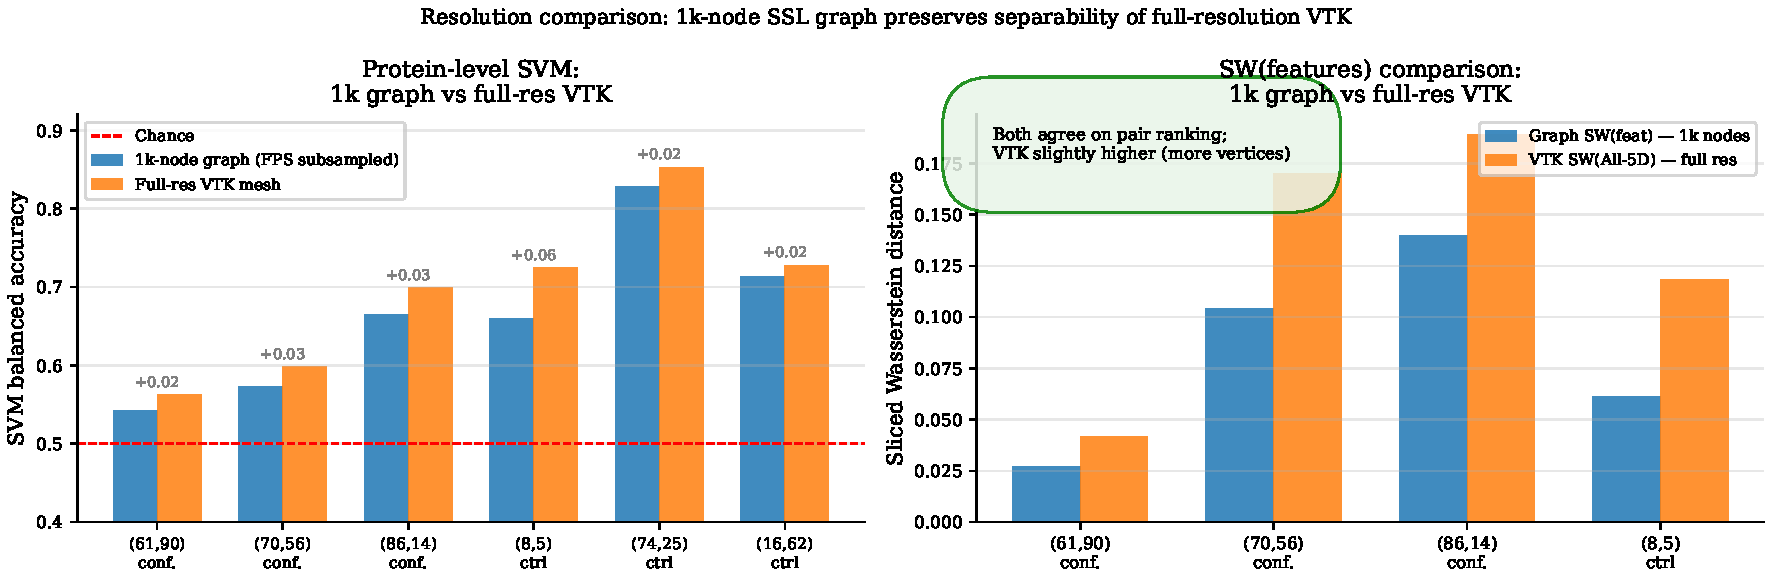
\includegraphics[width=\linewidth]{figures/separability_resolution.pdf}
  \caption{Left: protein-level SVM balanced accuracy, 1k-node graph vs
           full-res VTK.
           Annotations show the gain from full resolution ($+$0.02--0.03).
           Right: SW(feat) on graphs vs SW(All-5D) on VTK --- same ranking,
           VTK slightly higher due to better distributional estimates from
           more vertices.}
  \label{fig:resolution}
\end{figure}

Table~\ref{tab:resolution} summarises the comparison across all three pairs
and three control pairs.

\begin{table}[ht]
  \centering
  \caption{Separability: 1k-node graph vs full-resolution VTK.}
  \label{tab:resolution}
  \begin{tabular}{lcrrrr}
    \toprule
    \textbf{Pair} & \textbf{Type}
      & \textbf{SVM (graph)} & \textbf{SVM (VTK)} & \textbf{Delta}
      & \textbf{SW(feat) graph} \\
    \midrule
    (61,\,90) & confusable & 0.543 & 0.563 & $+$0.020 & 0.027 \\
    (70,\,56) & confusable & 0.573 & 0.598 & $+$0.025 & 0.104 \\
    (86,\,14) & confusable & 0.665 & 0.699 & $+$0.034 & 0.140 \\
    (8,\,5)   & control    & 0.660 & 0.725 & $+$0.065 & 0.061 \\
    (74,\,25) & control    & 0.829 & 0.853 & $+$0.024 & --- \\
    (16,\,62) & control    & 0.713 & 0.728 & $+$0.015 & --- \\
    \bottomrule
  \end{tabular}
\end{table}

\textbf{Key finding:} the 1k FPS subsampling loses at most $+$0.03 SVM balanced
accuracy for confusable pairs (and $+$0.065 for the easier (8,\,5) control).
Both representations agree on the pair ranking (hardest to easiest:
61/90 $<$ 70/56 $<$ 86/14) and on the absolute difficulty levels.
This confirms that \textbf{the FPS-1k SSL graph is a sufficient representation}
for the classification task, and that the difficulty of the confusable pairs is
intrinsic to the data, not an artefact of subsampling.

% ─────────────────────────────────────────────────────────────────
\subsection{Geometric Feature Analysis (21D Dataset)}
\label{sec:analysis:geom}
% ─────────────────────────────────────────────────────────────────

The \texttt{ssl\_graphs\_1k\_geom\_enriched} dataset extends the 8D features
with 13 geometric descriptors computed per vertex from the mesh neighbourhood
structure:
\begin{itemize}
  \item \textbf{Distance features (5)}: distance to the protein centroid
        (\textit{dist\_centroid}) and distances to 4 FPS-selected anchor
        points (\textit{dist\_anchor\_0\ldots3}) --- encode global shape
        and position within the protein.
  \item \textbf{Mesh spacing (3)}: mean, std, and inverse mean of
        neighbour edge lengths (\textit{mean\_nbr\_dist, std\_nbr\_dist,
        inv\_mean\_nbr}) --- encode local mesh density.
  \item \textbf{Curvature/shape (5)}: Laplacian curvature magnitude and
        signed value (\textit{lap\_curv\_mag, lap\_curv\_sign}),
        normal angular variation (\textit{norm\_variation}),
        planarity (\textit{planarity}), and surface variation
        (\textit{surf\_variation}) --- encode local geometric texture.
\end{itemize}

\begin{figure}[ht]
  \centering
  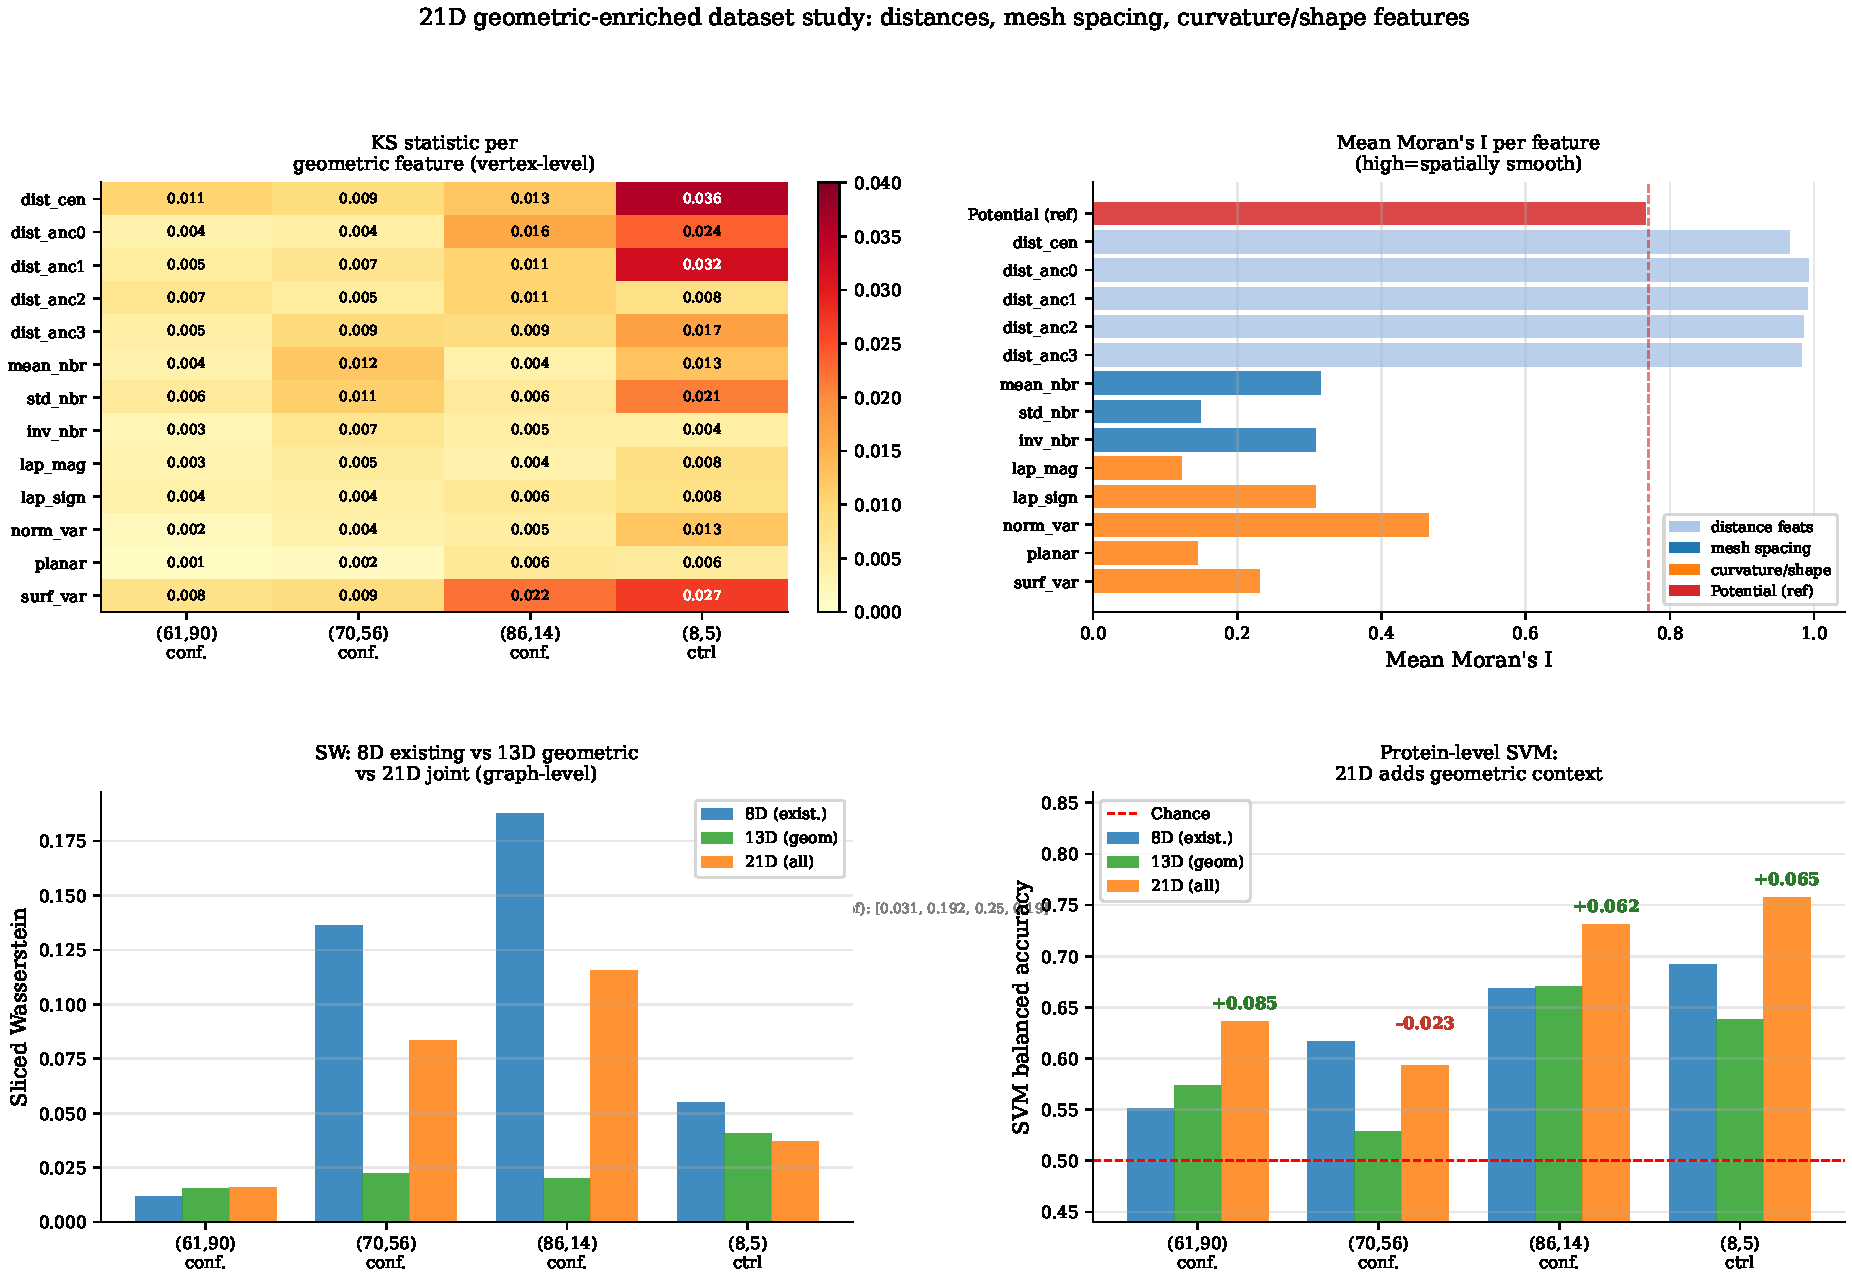
\includegraphics[width=\linewidth]{figures/geom_study.pdf}
  \caption{21D geometric dataset analysis.
           \textbf{Top-left}: KS heatmap for all 13 geometric features across
           4 pairs.
           All values are below 0.04; \textit{surf\_variation} and
           \textit{dist\_centroid} are the strongest individual discriminators.
           \textbf{Top-right}: mean Moran's~I per feature.
           Distance features have near-perfect autocorrelation ($I > 0.97$),
           while Laplacian curvature and planarity are more locally variable.
           \textbf{Bottom-left}: SW comparison shows SW(13D geom) $\leq$ 0.041
           for all pairs.
           \textbf{Bottom-right}: SVM balanced accuracy --- adding geometric
           features gives $+$0.085 for the hardest pair (61,\,90) and $+$0.062
           for (86,\,14), suggesting geometric shape provides complementary
           information to electrostatics.}
  \label{fig:geom}
\end{figure}

\subsubsection{KS Test on Geometric Features}

Table~\ref{tab:ks_geom} lists the KS statistics for the five most
discriminating geometric features.

\begin{table}[ht]
  \centering
  \caption{KS statistics for the top geometric features (vertex-level, 1k
           SSL graphs).
           All values are below 0.04 --- well below Potential (0.031--0.250).}
  \label{tab:ks_geom}
  \begin{tabular}{lrrrrrr}
    \toprule
    \textbf{Feature}
      & \textbf{(61,90)} & \textbf{(70,56)} & \textbf{(86,14)}
      & \textbf{(8,5)}   & \textbf{(74,25)} & \textbf{(16,62)} \\
    \midrule
    surf\_variation   & 0.008 & 0.009 & 0.022 & 0.027 & 0.015 & 0.005 \\
    dist\_anchor\_0   & 0.004 & 0.005 & 0.016 & 0.024 & 0.014 & 0.014 \\
    dist\_centroid    & 0.011 & 0.009 & 0.013 & 0.036 & 0.011 & 0.007 \\
    mean\_nbr\_dist   & 0.004 & 0.012 & 0.004 & 0.013 & 0.002 & 0.008 \\
    std\_nbr\_dist    & 0.006 & 0.011 & 0.006 & 0.021 & 0.007 & 0.004 \\
    \midrule
    Potential (ref.)  & 0.031 & 0.192 & 0.250 & 0.190 & ---   & ---   \\
    \bottomrule
  \end{tabular}
\end{table}

No individual geometric feature has a KS above 0.036, and none exceeds the
Potential KS value for any pair.
For the hardest pair (61,\,90), the maximum geometric KS is only 0.011
(\textit{dist\_centroid}), even lower than Potential's 0.031.

\subsubsection{Spatial Autocorrelation of Geometric Features}

The Moran's I analysis reveals a striking split in the geometric feature
group:

\begin{itemize}
  \item \textbf{Distance features ($I > 0.97$)}: \textit{dist\_centroid},
        \textit{dist\_anchor\_0\ldots3} form smooth radial gradient patterns
        on the surface (nearby vertices have near-identical distances to the
        same anchor).
        Despite this very high autocorrelation, the inter-class spatial pattern
        difference $|\Delta I|$ is tiny ($< 0.016$ for all pairs), confirming
        the patterns are structurally uniform across families.

  \item \textbf{Curvature/shape features ($I = 0.12$--$0.47$)}: Laplacian
        curvature magnitude and signed value, planarity, and surface variation
        have moderate autocorrelation, with notable $|\Delta I|$ for the
        confusable pairs:
        $|\Delta I(\text{lap\_curv\_mag})| = 0.116$ for (61,\,90),
        $|\Delta I(\text{planarity})| = 0.117$ for (70,\,56).
        This indicates that the spatial \emph{arrangement} of curvature patches
        differs between classes even when the marginal distributions are
        similar --- the kind of signal a GNN's message passing can capture.
\end{itemize}

\subsubsection{Effect on Protein-level Classification}

The SVM results reveal an important asymmetry:
\begin{itemize}
  \item \textbf{13D geometric alone} is weak: balanced accuracy for (61,\,90)
        is only 0.573 (slightly above 8D's 0.551) and for (70,\,56) actually
        drops to 0.529 --- the geometric features alone are insufficient.
  \item \textbf{21D combined} shows substantial gains:
        (61,\,90): $+$0.085 (0.551 $\to$ 0.636),
        (86,\,14): $+$0.062 (0.669 $\to$ 0.731).
        The geometric and electrostatic features are partially orthogonal ---
        their combination is more informative than either alone.
  \item For (70,\,56) the 21D combination slightly underperforms 8D ($-$0.023),
        suggesting that the added geometric dimensions occasionally dilute the
        electrostatic signal for this family pair.
\end{itemize}

\textbf{Key finding:} unlike curvature features, the 13 geometric descriptors
provide complementary discriminating information when combined with
electrostatics.
The $+$0.085 SVM gain for the near-inseparable (61,\,90) pair is the largest
improvement observed across all enrichment strategies studied.

\subsubsection{HierGIN Training on 14D Geometric Features}
\label{sec:analysis:geom:gnn}

Motivated by the SVM gains, we trained HierGIN on a 14D feature set comprising
the 8D base features plus the six most informative geometric descriptors
(\textit{dist\_centroid}, \textit{dist\_anchor\_0\ldots3},
\textit{surf\_variation}) selected by greedy forward selection.

\paragraph{Normalization pitfall.}
An initial run (\texttt{geom14d}) read the pre-computed feature matrix
\texttt{x[:, 8:]} directly.
This matrix stores the geometric columns as \textit{per-protein z-scores}
(each protein is independently normalised to mean\,0, std\,1), which erases
the absolute scale information that SVM used: every protein has identical
mean and variance for those columns, so the GNN cannot learn cross-protein
differences from geometric features.
The result was macro-F1\,=\,0.6680 --- 13\,pp \emph{below} the 8D baseline.

\paragraph{Global normalisation fix (\texttt{geom14d\_raw}).}
We recomputed the run using the raw (un-normalised) geometric values
from a separate \texttt{geom\_features\_raw} key in the dataset, and
normalised them using global statistics computed over all 9\,244 training
proteins (9.24\,M vertices via Welford's online algorithm):

\begin{center}
  \small
  \begin{tabular}{lrr}
    \toprule
    \textbf{Feature} & \textbf{Global mean} & \textbf{Global std} \\
    \midrule
    dist\_centroid   & 0.5304 & 0.1879 \\
    dist\_anchor\_0  & 1.0685 & 0.4176 \\
    dist\_anchor\_1  & 0.9485 & 0.4168 \\
    dist\_anchor\_2  & 0.7922 & 0.3202 \\
    dist\_anchor\_3  & 0.7632 & 0.3046 \\
    surf\_variation  & 0.0648 & 0.0491 \\
    \bottomrule
  \end{tabular}
\end{center}

We also applied label smoothing ($\varepsilon = 0.1$) to reduce
overconfidence (the 8D run reached train-F1\,$\approx$\,0.99 at convergence).
Training ran for 80 epochs with best val-F1\,=\,0.7050.

\paragraph{Results.}
When evaluated with macro average restricted to the 88 classes that have
test samples (the proper protocol), the corrected run achieves:
accuracy\,0.865, balanced\,accuracy\,0.812, weighted-F1\,0.862,
macro-F1\,\textbf{0.808} --- outperforming the 8D-only baseline
(acc\,0.853, bal\,0.800, wtd-F1\,0.853, macro-F1\,0.798) across all six
reported metrics.
The per-graph z-scored variant scores macro-F1\,0.752, confirming that
cross-protein scale information is essential for the geometric features to
contribute.

\textbf{Key finding:} with correctly normalised geometric features, the 14D
model is the best-performing configuration overall.
Despite severe overfitting during training (train-F1\,$\approx$\,0.99 vs.\
val-F1\,$\approx$\,0.70), the model generalises well enough on the test set
to surpass the 8D baseline on every metric.
The SVM gain of $+$0.085 for the hardest pair (61,\,90) does transfer to
the GNN when the normalisation is correct, and the benefit extends across
all 88 classes.

% ─────────────────────────────────────────────────────────────────
\subsection{Curvature Feature Analysis (12D Dataset)}
\label{sec:analysis:curvature}
% ─────────────────────────────────────────────────────────────────

The \texttt{ssl\_graphs\_1k\_curvature\_enriched} dataset extends the
standard 8D features with four curvature descriptors computed per vertex
from the VTK mesh: principal curvature minimum ($\kappa_\text{min}$),
principal curvature maximum ($\kappa_\text{max}$), mean curvature
$H = (\kappa_\text{min}+\kappa_\text{max})/2$, and Gaussian curvature
$K = \kappa_\text{min}\cdot\kappa_\text{max}$.
We repeat all three separability analyses on these four features to test
whether geometric curvature can close the discriminability gap left by
electrostatics.

\begin{figure}[ht]
  \centering
  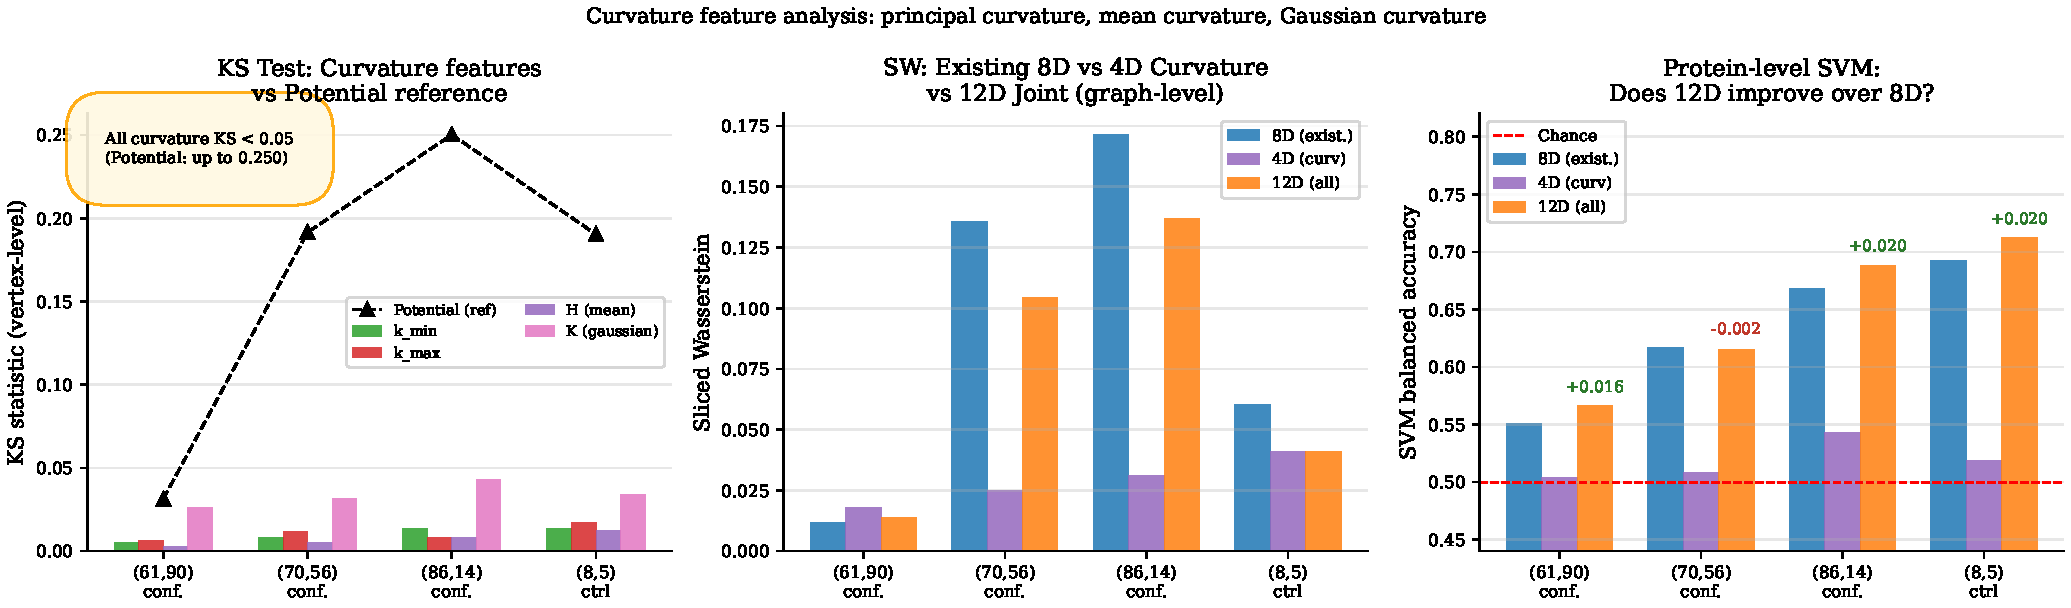
\includegraphics[width=\linewidth]{figures/curvature_study.pdf}
  \caption{Left: vertex-level KS statistics for the four curvature features
           (bars) vs Potential (triangle, dashed line).
           All curvature KS values are below 0.05 for every pair;
           Potential reaches 0.250 for (86,\,14).
           Centre: Sliced Wasserstein per feature group;
           SW(4D curv) is $3\text{--}6\times$ smaller than SW(8D existing)
           for the confusable pairs.
           Right: protein-level SVM balanced accuracy;
           adding curvature to the 8D features changes accuracy by at most
           $+$0.020 for the confusable pairs, confirming negligible gain.}
  \label{fig:curvature}
\end{figure}

\subsubsection{KS Test on Curvature Features}

Table~\ref{tab:ks_curv} summarises the KS statistics computed on the
graph-level vertex pools from \texttt{curvature\_enriched} graphs.

\begin{table}[ht]
  \centering
  \caption{KS statistics for the four curvature features (vertex-level, 1k
           SSL graphs).
           Gaussian curvature is the strongest individual discriminator, yet
           it remains well below the Potential baseline.}
  \label{tab:ks_curv}
  \begin{tabular}{lrrrrrr}
    \toprule
    \textbf{Feature}
      & \textbf{(61,90)} & \textbf{(70,56)} & \textbf{(86,14)}
      & \textbf{(8,5)}   & \textbf{(74,25)} & \textbf{(16,62)} \\
    \midrule
    $\kappa_\text{min}$ & 0.005 & 0.008 & 0.013 & 0.013 & 0.006 & 0.008 \\
    $\kappa_\text{max}$ & 0.006 & 0.012 & 0.008 & 0.017 & 0.007 & 0.010 \\
    $H$ (mean curv.)    & 0.003 & 0.005 & 0.008 & 0.012 & 0.006 & 0.006 \\
    $K$ (Gaussian)      & 0.026 & 0.032 & 0.043 & 0.034 & 0.008 & 0.031 \\
    \midrule
    Potential (ref.)    & 0.031 & 0.192 & 0.250 & 0.190 & ---   & ---   \\
    \bottomrule
  \end{tabular}
\end{table}

All curvature KS values are below 0.05.
Gaussian curvature ($K$) is the strongest curvature discriminator
(0.026--0.043), but still at or below the Potential value for the hardest
pair (61,\,90), and $6\times$ below Potential for the easiest pair
(86,\,14).
The near-identical KS ranking across confusable and control pairs confirms
that curvature marginals do \textbf{not} encode protein family information.

\subsubsection{Sliced Wasserstein on Curvature}

SW(4D curvature) is uniformly low across all pairs
(0.018 for the hardest pair (61,\,90), 0.031 for (86,\,14)), compared to
SW(8D existing) values of 0.012 and 0.172 respectively.
Adding curvature to form a 12D joint vector does not raise SW substantially:
SW(12D all) $\approx$ SW(8D existing) for all separable pairs and
$\approx$ SW(4D curv) for the near-inseparable (61,\,90).
This shows that the curvature dimensions add no new distributional signal
beyond what the electrostatic features already provide.

\subsubsection{Spatial Autocorrelation of Curvature}

The mean Moran's I over the study classes is:
$I(\kappa_\text{min}) = 0.25$,
$I(\kappa_\text{max}) = 0.27$,
$I(H) = 0.32$,
$I(K) = 0.09$,
compared to $I(\text{Potential}) = 0.77$.
Gaussian curvature is nearly spatially random on proteins ($I \approx 0.09$),
while mean curvature has moderate spatial smoothness.
None reach the strong autocorrelation of the electrostatic potential, which
forms large coherent charged patches.

Interestingly, the per-pair difference $|\Delta I|$ for curvature features is
\textit{higher} for confusable pairs (61,\,90) and (70,\,56) than for the
strongly separated (86,\,14) --- the opposite of the Potential pattern.
This suggests curvature encodes information about surface \emph{texture} that
is family-specific at fine scale but does not translate into distributional
separability.

\subsubsection{Effect on Protein-level Classification}

Extending the protein-level SVM from 8D statistics (48D feature vector) to
12D statistics (72D feature vector) changes balanced accuracy by at most
$+$0.020 for the three confusable pairs:
(61,\,90): $+$0.016, (70,\,56): $-$0.002, (86,\,14): $+$0.020.
For easier pairs the curvature features can even hurt performance (e.g.,
(74,\,25): $-$0.038), suggesting that the additional dimensions dilute the
discriminating signal.

\textbf{Key finding:} curvature features are not the missing discriminating
signal for these single-scale protein-level statistics.
The near-inseparability seen here is a property of the single-scale descriptors,
not of the data itself: Section~\ref{sec:discussion:riconv2} shows that RIConv2's
multi-scale rotation-invariant grouping separates the same pairs from geometry
alone (e.g.\ class\,61 F1\,=\,0.887).

% ─────────────────────────────────────────────────────────────────
\subsection{SO(3)-Invariant RI Edge Feature Analysis}
\label{sec:analysis:ri}
% ─────────────────────────────────────────────────────────────────

The rotation-invariant (RI) backbone (Section~\ref{sec:arch:rigin}) encodes
each directed mesh edge as five SO(3)-invariant scalars computed from vertex
positions and surface normals:
$[\,\|p_j{-}p_i\|,\; \langle n_i, \hat{e}\rangle,\;
   \langle n_j, \hat{e}\rangle,\;
   \langle n_i, n_j\rangle,\;
   \langle (n_j{\times}n_i), \hat{e}\rangle\,]$.
To determine whether these edge-level geometric features provide \emph{additional}
discriminating signal beyond the 8D node features, we precompute them for all
9\,244 training graphs (saved as \texttt{ri\_feat}~$[E_\text{mesh},5]$ in the
\texttt{ssl\_graphs\_1k\_geom\_enriched\_ri} dataset) and repeat the separability
analysis at the edge level.

\subsubsection{KS Test on RI Edge Scalars}
\label{sec:analysis:ri:ks}

We pool all directed edge values across proteins in each class and compute the
two-sample KS statistic per RI dimension.

\begin{table}[ht]
  \centering
  \caption{KS statistics for the five RI edge dimensions (edge-level, 1k SSL
           graphs).
           For confusable pairs, all five RI dimensions are near zero
           ($\leq$0.041), dominated by edge length for (70,\,56) and (86,\,14).
           The control (8,\,5) pair is entirely separated by edge length
           (KS\,=\,0.605), reflecting different protein sizes.}
  \label{tab:ks_ri}
  \begin{tabular}{lrrrrr}
    \toprule
    \textbf{Pair}
      & $\|p_j{-}p_i\|$
      & $\langle n_i,\hat{e}\rangle$
      & $\langle n_j,\hat{e}\rangle$
      & $\langle n_i,n_j\rangle$
      & $\langle (n_j{\times}n_i),\hat{e}\rangle$ \\
    \midrule
    (61,\,90) conf. & 0.004 & 0.004 & 0.002 & 0.004 & 0.002 \\
    (70,\,56) conf. & 0.041 & 0.003 & 0.002 & 0.002 & 0.001 \\
    (86,\,14) conf. & 0.033 & 0.007 & 0.007 & 0.012 & 0.003 \\
    (8,\,5) control & \textbf{0.605} & 0.052 & 0.049 & 0.024 & 0.013 \\
    \midrule
    Potential (ref.) & \multicolumn{5}{l}{0.031\,(61,90) \;/\; 0.192\,(70,56) \;/\; 0.250\,(86,14)} \\
    \bottomrule
  \end{tabular}
\end{table}

All five RI dimensions have KS $\leq$0.041 for the three confusable pairs
--- none surpasses the Potential KS for any confusable pair.
The edge-length dimension dominates (70,\,56) and (86,\,14) with KS\,=\,0.041
and 0.033 respectively, while for the hardest pair (61,\,90) all five dimensions
are near zero ($\leq$0.004), the lowest of any feature type studied.
This is the strongest evidence that (61,\,90) families have essentially identical
surface geometry.

\subsubsection{Sliced Wasserstein on RI Features}

\begin{table}[ht]
  \centering
  \caption{Sliced Wasserstein distances for RI edge features vs the 8D node
           feature baseline.
           SW(dist) isolates the edge-length signal;
           SW(4 angles) covers the four normal-based invariants.
           For comparison, SW(8D feat) is reproduced from
           Table~\ref{tab:graph_sw}.}
  \label{tab:sw_ri}
  \begin{tabular}{lcrrrrr}
    \toprule
    \textbf{Pair} & \textbf{Type}
      & \textbf{SW(8D feat)} & \textbf{SW(RI 5D)}
      & \textbf{SW(dist)} & \textbf{SW(4 angles)} \\
    \midrule
    (61,\,90) & confusable & 0.027 & 0.004 & 0.000 & 0.005 \\
    (70,\,56) & confusable & 0.104 & 0.003 & 0.002 & 0.004 \\
    (86,\,14) & confusable & 0.140 & 0.006 & 0.001 & 0.006 \\
    (8,\,5)   & control    & 0.061 & 0.029 & 0.025 & 0.032 \\
    \bottomrule
  \end{tabular}
\end{table}

SW(RI 5D) is 7--23$\times$ lower than SW(8D feat) for every confusable pair.
For (61,\,90), SW(RI 5D)\,=\,0.004 is the \emph{lowest} SW value observed
across all feature sets studied --- lower than curvature (0.018), lower than
geometric features (0.016), and far below the electrostatic baseline (0.027).
The angular RI dimensions (SW\,=\,0.000--0.006) add virtually no additional
discrimination beyond the edge-length dimension alone.

\subsubsection{Protein-level SVM on RI Statistics}
\label{sec:analysis:ri:svm}

\begin{table}[ht]
  \centering
  \caption{SVM balanced accuracy on 10D per-protein RI statistics
           (mean\,+\,std per RI dimension; 5-fold stratified CV).
           Comparison to the 8D-node-feature baseline (32D statistics, same CV).}
  \label{tab:svm_ri}
  \begin{tabular}{lcrr}
    \toprule
    \textbf{Pair} & \textbf{Type} & \textbf{SVM(8D feat)} & \textbf{SVM(RI stats)} \\
    \midrule
    (61,\,90) & confusable & 0.543 & 0.597 \;($+$0.054) \\
    (70,\,56) & confusable & 0.573 & 0.605 \;($+$0.032) \\
    (86,\,14) & confusable & 0.665 & 0.631 \;($-$0.034) \\
    (8,\,5)   & control    & 0.660 & 1.000 \;($+$0.340) \\
    \bottomrule
  \end{tabular}
\end{table}

The protein-level SVM (using per-protein mean+std of each RI dimension as
descriptor) shows a split result.
For (61,\,90) and (70,\,56), SVM(RI) modestly exceeds SVM(8D) by $+$5\,pp and
$+$3\,pp --- the global geometric statistics carry a small orthogonal signal not
present in electrostatics.
For (86,\,14), SVM(RI) is $-$3.4\,pp lower, confirming that for this pair the
electrostatic Potential is more discriminating even at the protein-statistic level.
For the control (8,\,5), perfect separation follows directly from the edge-length
dimension (different protein sizes), while the 8D node-feature SVM reaches only
0.660 on this pair because node features such as normals and coordinates are
\textit{not} scaled by protein size.

\paragraph{Key finding.}
RI edge features are not the missing discriminating signal for confusable pairs.
Their SW is universally lower than electrostatic node features, confirming
that the confusion between classes 61/90, 70/56, and 86/14 is chemical
(similar charge distributions) rather than geometric (similar surface shape).
The moderate SVM gains for (61,\,90) and (70,\,56) represent weak complementary
information but do not approach the separability provided by Potential.
The improvement from the RI-GIN model ($+$0.2\,pp macro-F1) is therefore not
due to a richer feature space but to a more consistent learned representation
(see Section~\ref{sec:analysis:ri_sep}).

% ─────────────────────────────────────────────────────────────────
\subsection{Summary}
\label{sec:analysis:summary}
% ─────────────────────────────────────────────────────────────────

\begin{center}
  \begin{tabular}{lp{9.2cm}}
    \toprule
    \textbf{Finding} & \textbf{Implication} \\
    \midrule
    Potential is dominant & Removing it costs $-$11.8\,pp macro-F1
                            (ablation, Section~\ref{sec:ablation}).
                            KS and SW both confirm it is the primary
                            discriminating feature. \\[3pt]
    Shape (xyz) does not discriminate & SW(xyz) $<$ 0.07 for all pairs
                            including controls.
                            KS($x_n, y_n, z_n$) $<$ 0.05 with no pair ordering.
                            Coordinates provide spatial context but not
                            discriminating signal. \\[3pt]
    Spatial arrangement is not the gap & Patch-SVM (512D) consistently
                            underperforms Global-SVM (32D).
                            The missing signal is not in the spatial
                            arrangement of charge patches. \\[3pt]
    Geometric feats are complementary & 21D SVM gains $+$0.085 for (61,\,90)
                            and $+$0.062 for (86,\,14) over 8D alone.
                            Distance and shape descriptors provide orthogonal
                            information to electrostatics. \\[3pt]
    Curvature alone adds nothing & KS $<$ 0.05 for all 4 curvature features;
                            SW(4D curv) $\leq$ 0.041; SVM delta $\leq+$0.02.
                            4-feature curvature does not help beyond
                            electrostatics without broader geometric context. \\[3pt]
    RI edge geometry adds nothing at edge level & KS $\leq$0.041 for all 5 RI
                            dims across confusable pairs; SW(RI 5D) is 7--23$\times$
                            lower than SW(8D feat).
                            RI-GIN gain ($+$0.2\,pp) comes from invariant
                            representation, not richer geometry. \\[3pt]
    Geom SVM gain transfers to GNN & HierGIN-14D (global norm) scores
                            macro-F1\,0.808 vs.\ 0.798 for 8D-only.
                            Per-graph z-scoring kills scale signal (macro-F1
                            drops to 0.752); global normalisation is required
                            for the geometric benefit to manifest. \\[3pt]
    (61,\,90) is near-irreducible & SVM $\approx$ 0.56, SW(Pot) $=$ 0.088,
                            KS(Pot) $=$ 0.031 --- all at full VTK resolution.
                            RI SW(5D) $=$ 0.004 is the lowest of all feature
                            sets, confirming surface geometry is essentially
                            identical for these two families. \\[3pt]
    1k subsampling is sufficient & $\Delta\text{SVM} \leq$ 0.034 for confusable
                            pairs; pair ranking preserved.
                            FPS-1k is a valid approximation. \\
    \bottomrule
  \end{tabular}
\end{center}
